\documentclass{beamer}

% Packages
\usepackage{graphicx}
\usepackage{subcaption}
\usepackage{amsmath, amssymb}
\usepackage{listings}
\usepackage{xcolor}

\usepackage[backend=bibtex]{biblatex}
\bibliography{ref}

\DeclareCiteCommand{\cite}
{\usebibmacro{prenote}}
{\usebibmacro{citeindex}%
	\printtext[bibhyperref]{\color{blue}\mkbibbrackets{\usebibmacro{cite}}}}
{\multicitedelim}
{\usebibmacro{postnote}}



% Title and Author Information
\title{Introduction to Optimal Transport and its Applications to Computational Biology}
\author{{Anthony Christidis}}
\institute{
	\normalsize
	Journal Club\\
	Computational Biology Group\\[0.4cm]
	Core for Computational Biology\\
	Department of Biomedical Informatics\\
	Harvard Medical School
}
\date{
	January 23, 2025  % Automatically inserts the current date
}


\begin{document}
	
	% Title Slide
	\begin{frame}
		\titlepage
		\begin{center}
			
\includegraphics[width=0.4\textwidth]{HMS_DBMI_Logo.png}
		\end{center}
	\end{frame}
	
	% Outline
	\begin{frame}
		\frametitle{Outline}
		\tableofcontents
	\end{frame}
	
	% Basics of Optimal Transport
	\begin{frame}
		\frametitle{Relevant Materials}
		\begin{itemize}
			\item \textbf{Theoretical and Computational Optimal Transport}:
			\begin{itemize}
				\item "\textbf{Optimal transport for single-cell and spatial omics}`` by Charlotte Bunne, Geoffrey Schiebinger, Andreas Krause, Aviv Regev and Marco Cuturi. \cite{bunne2024optimal}
				\item "\textbf{Computational Optimal Transport}`` by Gabriel Peyré and Marco Cuturi. \cite{peyre2019computational}
				\item "\textbf{Optimal Transport for Applied Mathematicians}`` by Filippo Santambrogio. \cite{santambrogio2015optimal}
			\end{itemize}
			\item \textbf{Software Packages}:
			\begin{itemize}
				\item \texttt{transport} \cite{transport}
				\item \texttt{POT} \cite{flamary2021pot}
				\item \texttt{scDiagnostics} \cite{scDiagnostics}
			\end{itemize}
		\end{itemize}
	\end{frame}
	
	\section{Basics of Optimal Transport}
	\begin{frame}
		\frametitle{Basics of Optimal Transport}
		\begin{itemize}
			\item Optimal Transport (OT) focuses on the most efficient way to move mass between distributions.
			\item Connections to diverse fields: probability, statistics, optimization, functional analysis, and many more.
		\end{itemize}
		\begin{figure}
			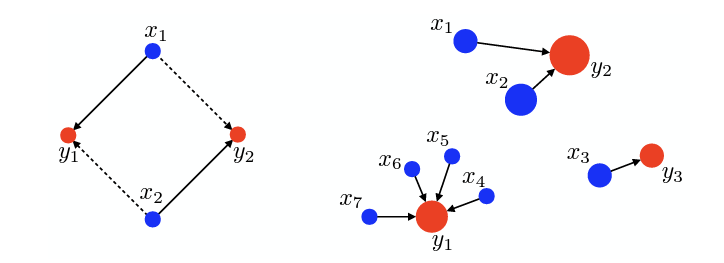
\includegraphics[width=0.8\textwidth]{basics.png}
			\caption{Example discrete OT problem solutions. \cite{peyre2019computational}}
		\end{figure}
	\end{frame}
	
	\begin{frame}
		\frametitle{Basics of Optimal Transport}
		\begin{itemize}
			\item Areas of applications: \textbf{computational biology}, image processing, economics, and many more.
		\end{itemize}
		\begin{figure}
			\begin{subfigure}{0.4\textwidth}
				\centering
				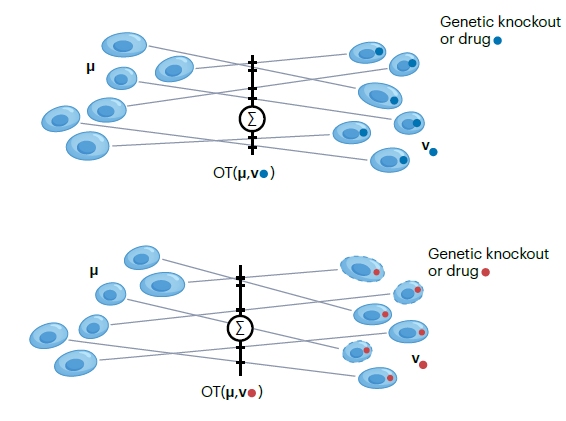
\includegraphics[width=\textwidth]{comp_bio.png}
				\caption{Computational Biology \cite{bunne2024optimal}}
			\end{subfigure}
			\hfill
			\begin{subfigure}{0.4\textwidth}
				\centering
				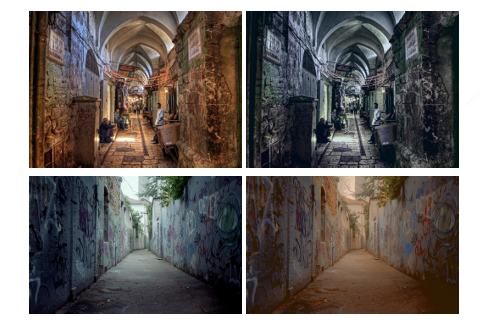
\includegraphics[width=\textwidth]{image_processing.png}
				\caption{Image Processing \cite{santambrogio2015optimal}}
			\end{subfigure}
			
			\begin{subfigure}{0.8\textwidth}
				\centering
				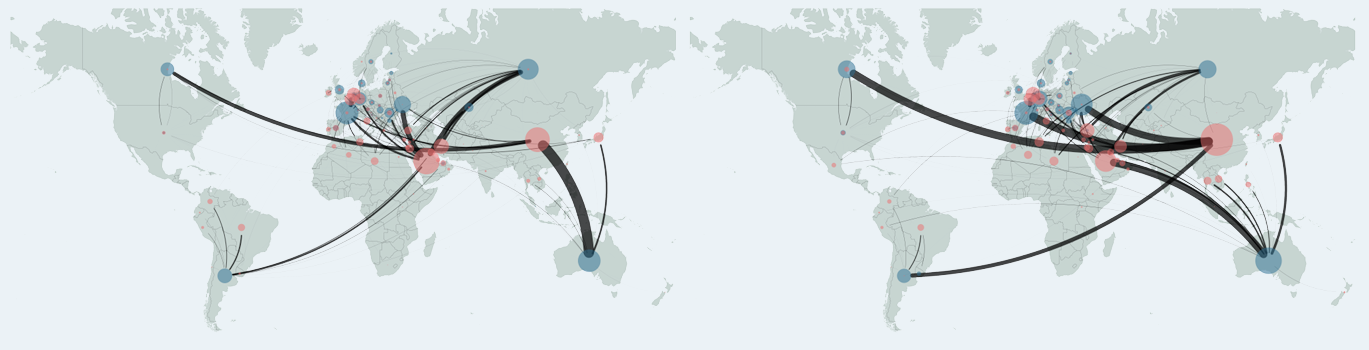
\includegraphics[width=\textwidth]{economics.png}
				\caption{Economics \cite{gaskin2024modelling}}
			\end{subfigure}
		\end{figure}
	\end{frame}
	
	\begin{frame}
		\frametitle{Basics of Optimal Transport}
		\begin{itemize}
			\item Fundamental problem: Moving mass from one distribution to another at minimal cost.
		\end{itemize}
		\begin{figure}
			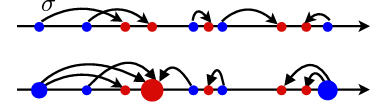
\includegraphics[width=0.8\textwidth]{fundamental_problem.png}
			\caption{Fundamental problem in OT. \cite{peyre2019computational}}
		\end{figure}
	\end{frame}
	
	% Discrete Optimal Transport
	\section{Discrete Optimal Transport}
	
	% Mathematical Background
	\subsection{Mathematical Background}
	\begin{frame}
		\frametitle{Discrete OT: Mathematical Background}
		\begin{itemize}
			\item \textbf{Source Distribution} (\(\mu\)): \(\mu = \sum_{i=1}^n a_i \delta_{x_i}\)
			\begin{itemize}
				\item \(a_i\): Mass or probability at source point \(x_i\).
				\item \(\delta_{x_i}\): Dirac delta function, representing mass concentrated at \(x_i\).
			\end{itemize}
			
			\item \textbf{Target Distribution} (\(\nu\)): \(\nu = \sum_{j=1}^m b_j \delta_{y_j}\)
			\begin{itemize}
				\item \(b_j\): Mass or probability at target point \(y_j\).
				\item \(\delta_{y_j}\): Dirac delta function, representing mass concentrated at \(y_j\).
			\end{itemize}
			\item \textbf{Dirac Delta Function} (\(\delta_{x_i}\)):
			\begin{itemize}
				\item Models an idealized point mass.
			\end{itemize}
			
			\item \textbf{Measure Theory}:
			\begin{itemize}
				\item Studies objects like \(\mu\) and \(\nu\), defines how mass is distributed.
			\end{itemize}
		\end{itemize}
		\begin{figure}
			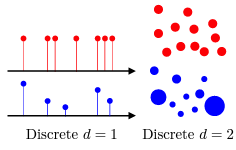
\includegraphics[width=0.35\textwidth]{discrete.png}
			\caption{Example of probability mass functions. \cite{peyre2019computational}}
		\end{figure}
	\end{frame}
	
	\begin{frame}
		\frametitle{Discrete OT: Transport Plan and Objective}
		\begin{itemize}
			\item \textbf{Transport Plan} (\(\pi\)): Matrix \(\pi_{ij}\) representing mass flow from \(x_i\) to \(y_j\).
			\item \textbf{Objective}:
			\[
			\min \sum_{i=1}^n \sum_{j=1}^m \pi_{ij} c(x_i, y_j)
			\]
			\item \textbf{Constraints}:
			\begin{align*}
				&\sum_{j=1}^m \pi_{ij} = a_i, \quad \forall i \\
				&\sum_{i=1}^n \pi_{ij} = b_j, \quad \forall j \\
				&\pi_{ij} \geq 0, \quad \forall i, j
			\end{align*}
			\item Cost function \(c(x_i, y_j)\) is often the squared distance \(\|x_i - y_j\|^2\).
		\end{itemize}
	\end{frame}
	
	\begin{frame}
		\frametitle{Entropy Regularization in Discrete OT}
		\begin{itemize}
			\item \textbf{Objective with Entropy Regularization}: Enhances computational efficiency and stability.
			\[
			\min_{\pi} \left( \sum_{i=1}^n \sum_{j=1}^m \pi_{ij} c(x_i, y_j) + \epsilon \sum_{i=1}^n \sum_{j=1}^m \pi_{ij} (\log \pi_{ij} - 1) \right)
			\]
			\begin{itemize}
				\item \(\epsilon\): Regularization tuning parameter.
			\end{itemize}
			
			\item \textbf{Benefits of Regularization}:
			\begin{itemize}
				\item Induces sparsity in \(\pi\).
				\item Improves numerical stability in high-dimensional problems.
				\item Faster convergence in optimization problems.
			\end{itemize}
			
			\item \textbf{Optimization Methods}:
			\begin{itemize}
				\item {Sinkhorn-Knopp Algorithm}
				
				\item {Other Methods}: iterative Bregman projections, stochastic optimization, augmented lagrangian methods
			\end{itemize}
		\end{itemize}
	\end{frame}
	
	\begin{frame}
		\frametitle{Discrete OT: Dual Formulation}
		\begin{itemize}
			\item The dual formulation involves maximizing:
			\[
			\sum_{i=1}^n u_i a_i + \sum_{j=1}^m v_j b_j
			\]
			\item Subject to:
			\[
			u_i + v_j \leq c(x_i, y_j) \quad \forall i, j
			\]
			\item Provides a complementary perspective on the transport problem.
		\end{itemize}
	\end{frame}
	
	\begin{frame}
		\frametitle{Monge vs. Kantorovich in OT}
		\begin{itemize}
			\item \textbf{Monge Problem}: Seeks a deterministic map \(T\) with \(T_\# \mu = \nu\), i.e. a bijective mapping with no splitting (so it has more constraints than the traditional/Kantorovich OT).
			\item \textbf{Kantorovich Problem}: Uses a transport plan \(\pi\) allowing mass splitting.
			\item Kantorovich is more flexible and widely applicable, handling broader cases where direct mappings (as in Monge) aren't possible.
			\item Monge required more computationally intensive methods from combinatorics.
		\end{itemize}
	\end{frame}
	
	% Example
	\subsection{Two Basic Examples}
		
		\begin{frame}
			\frametitle{Monge Problem Example}
			\begin{itemize}
				\item \textbf{Source Points}: \( \{x_1, x_2, x_3, x_4, x_5\} \)
				\item \textbf{Target Points}: \( \{y_1, y_2, y_3, y_4, y_5\} \)
				\item \textbf{Complex Cost Function}:
				\[
				\text{Cost}(x_i, y_j) = (i - j)^2 + 2i + 3j
				\]
				\item \textbf{Objective}: Find a mapping \(T: X \to Y\) minimizing the cost.
			\end{itemize}
			\begin{figure}
				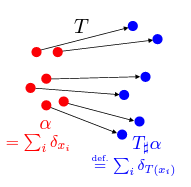
\includegraphics[width=0.25\textwidth]{monge.png}
				\caption{Bijective mapping example. \cite{peyre2019computational}}
			\end{figure}
		\end{frame}
		
		\begin{frame}
			\frametitle{Comparison of Solutions}
			\textbf{Solution 1}:
			\begin{align*}
				T(x_1) &= y_3, T(x_2) &= y_4, T(x_3) &= y_5, T(x_4) &= y_1, T(x_5) &= y_2
			\end{align*}
			\textbf{Total Cost for Solution 1}:
			\begin{itemize}
				\item Cost  = 102
			\end{itemize}
			
			\vspace{0.5cm}
			
			\textbf{Solution 2}:
			\begin{align*}
				T(x_1) &= y_2, T(x_2) &= y_3, T(x_3) &= y_4, T(x_4) &= y_5, T(x_5) &= y_1
			\end{align*}
			\textbf{Total Cost for Solution 2}:
			\begin{itemize}
				\item Cost  = 98
			\end{itemize}
			
			\vspace{0.5cm}
			
			\textbf{Conclusion}:
			\begin{itemize}
				\item Solution 2 has lower cost (98) compared to Solution 1 (102).
				\item Finding the optimal solution is very computationally expensive.
			\end{itemize}
		\end{frame}
		
		\begin{frame}
			\frametitle{Kantorovich Problem Example}
			\begin{itemize}
				\item \textbf{Source Points} with masses:
				\begin{itemize}
					\item \(x_1: 0.2\), \(x_2: 0.1\), \(x_3: 0.3\), \(x_4: 0.2\), \(x_5: 0.2\)
				\end{itemize}
				\item \textbf{Target Points} with masses:
				\begin{itemize}
					\item \(y_1: 0.15\), \(y_2: 0.25\), \(y_3: 0.25\), \(y_4: 0.15\), \(y_5: 0.2\)
				\end{itemize}
				\item \textbf{Cost Function}:
				\[
				\text{Cost}(x_i, y_j) = 
				\begin{cases} 
					1, & \text{if } i = j \\ 
					4, & \text{if } i \neq j 
				\end{cases}
				\]
				\item \textbf{Objective}: Minimize cost with transport plan allowing splits.
			\end{itemize}
		\end{frame}
		
		\begin{frame}
			\frametitle{Kantorovich Problem Solution}
			\textbf{Transport Plan (\(\pi\))}:
			\[
			\pi = \begin{bmatrix} 
				0.15 & 0.05 & 0 & 0 & 0 \\
				0 & 0.05 & 0.05 & 0 & 0 \\
				0 & 0.2 & 0.1 & 0 & 0 \\
				0 & 0 & 0.1 & 0.1 & 0 \\
				0 & 0 & 0 & 0.05 & 0.15 
			\end{bmatrix}
			\]
			\begin{itemize}
				\item Reflects optimal mass distribution.
				\item Allows splitting for more flexibility and lower cost.
				\item Calculation involves sum of \(\pi_{ij} \cdot \text{Cost}(x_i, y_j)\).
			\end{itemize}
		\end{frame}
	
	% Code Application
	\subsection{Code Applications}
	\begin{frame}
		\frametitle{Discrete OT: Code Applications}
		\begin{itemize}
			\item State-of-the-art solvers in R/CRAN package \texttt{transport}.
			\item See accompanying \texttt{R} script.
			\item Also available in Python via package POT.
		\end{itemize}
	\end{frame}
	
	% Continuous Optimal Transport
	\section{Continuous Optimal Transport}
	
	% Mathematical Background
	\subsection{Mathematical Background}
	\begin{frame}
		\frametitle{Continuous OT: Introduction}
		\begin{itemize}
			\item \textbf{Extension from Discrete to Continuous}:
			\begin{itemize}
				\item Generalizes optimal transport to manage continuous probability distributions.
				\item Useful for modeling and analyzing scenarios where data is naturally continuous.
			\end{itemize}
			
			\item \textbf{Source and Target Measures}:
			\begin{itemize}
				\item \(\mu\): Source measure, representing the initial "mass" distribution over space \(X\).
				\item \(\nu\): Target measure, representing the desired mass distribution over space \(Y\).
			\end{itemize}
		
		\end{itemize}
	\end{frame}
	
	\begin{frame}
		\frametitle{Continuous OT: Mathematical Formulation}
		\begin{itemize}
			\item \textbf{Transport Plan Set}:
			\begin{itemize}
				\item \(\Pi(\mu, \nu)\): Collection of all feasible transport plans \(\pi\) that shift \(\mu\) into \(\nu\) while conserving mass.
			\end{itemize}
			
			\item \textbf{Cost Function}:
			\begin{itemize}
				\item \(c(x, y)\): Represents the cost of moving a unit of mass from \(x \in X\) to \(y \in Y\).
			\end{itemize}
			
			\item \textbf{Objective}:
			\begin{itemize}
				\item Minimize total transport cost:
				\[
				\inf_{\pi \in \Pi(\mu, \nu)} \int_{X \times Y} c(x, y) \, d\pi(x, y)
				\]
				\item \(\inf\): Infimum, denotes the greatest lower bound of the total cost.
				\item \(\int_{X \times Y} c(x, y) \, d\pi(x, y)\): Integral, representing expected transport cost under plan \(\pi\).
			\end{itemize}
		\end{itemize}
	\end{frame}
	
	\begin{frame}
		\frametitle{Solving Continuous OT Problems}
		\begin{itemize}
			\item \textbf{Problem Setup}:
			\begin{itemize}
				\item Minimize integral-based cost:
				\[
				\inf_{\pi \in \Pi(\mu, \nu)} \int_{X \times Y} c(x, y) \, d\pi(x, y)
				\]
			\end{itemize}
			
			\item \textbf{Numerical Methods}:
			\begin{itemize}
				\item \textbf{Discretization}: Transform continuous measures into discrete approximations, linking directly to discrete OT techniques.
				\item \textbf{Sinkhorn-Knopp Algorithm}:
				\begin{itemize}
					\item Extends discrete OT regularization for efficiency.
				\end{itemize}
				\item \textbf{Gradient-Based Approaches}: Leverages derivatives to iteratively approach solutions.
			\end{itemize}
			
			\item \textbf{Theoretical Tools}:
			\begin{itemize}
				\item \textbf{Kantorovich Duality}: Bridges discrete and continuous OT solutions, using dual variables.
			\end{itemize}
			
			\item \textbf{Applications}: Extends discrete OT use cases in data science and ML.
		\end{itemize}
	\end{frame}
		
	
	% Example
	\subsection{One Basic Example}
	\begin{frame}
		\frametitle{Continuous OT Example: Problem Setup}
		\begin{itemize}
			\item \textbf{Source Distribution (\(\mu\))}:
			\begin{itemize}
				\item Gaussian centered at \((0, 0)\) with variance \(\Sigma_1 = I\) (identity matrix).
			\end{itemize}
			
			\item \textbf{Target Distribution (\(\nu\))}:
			\begin{itemize}
				\item Gaussian centered at \((1, 1)\) with variance \(\Sigma_2 = I\).
			\end{itemize}
			
			\item \textbf{Cost Function}:
			\begin{itemize}
				\item Squared Euclidean distance: \(c(x, y) = \|x - y\|^2\).
			\end{itemize}
			
			\item \textbf{Objective}:
			\begin{itemize}
				\item Find transport map \(T(x)\) that minimizes:
				\[
				\inf_{T} \int_{\mathbb{R}^2} \|x - T(x)\|^2 \, d\mu(x)
				\]
				\item Subject to mapping \(\mu\) to \(\nu\).
			\end{itemize}
		\end{itemize}
	\end{frame}
	
	\begin{frame}
		\frametitle{Continuous OT Example: Solution}
		\begin{itemize}
			\item \textbf{Optimal Transport Map via Brenier's Theorem}:
			\begin{itemize}
				\item For Gaussian distributions with quadratic cost, the map is affine:
				\[
				T(x) = Ax + b
				\]
				\item Given \(\Sigma_1 = \Sigma_2 = I\), set \(A = I\).
			\end{itemize}
			
			\item \textbf{Translation Vector (\(b\))}:
			\begin{itemize}
				\item Shift from source to target mean: 
				\[
				b = (1, 1) - (0, 0) = (1, 1)
				\]
			\end{itemize}
			
			\item \textbf{Result}:
			\begin{itemize}
				\item Optimal map: 
				\[
				T(x) = x + (1, 1)
				\]
				\item Each point is shifted right and up by 1 to align with \(\nu\).
			\end{itemize}
			
			\item \textbf{Explanation}:
			\begin{itemize}
				\item Map \(T(x)\) realigns means without variance adjustment, ideal for equal covariance identity matrices.
			\end{itemize}
		\end{itemize}
	\end{frame}
	
	
	% Code Application
	\subsection{Code Application}
	\begin{frame}
		\frametitle{Continuous OT: Code Application}
		\begin{itemize}
			\item See accompanying \texttt{R} script.
			\item In the continuous code example, we verify our intuition via simulation.
			\item See plot produced at the end of this example.
		\end{itemize}
	\end{frame}
	
	% Applications to Computational Biology
	\section{Applications to Computational Biology}
	
	% Applications to Single-Cell Omics
	\subsection{Applications to Single-Cell Omics}
	\begin{frame}
		\frametitle{Comparing Single-Cell Expressions: Traditional Metrics}
		\begin{itemize}
			\item \textbf{Limitations of Euclidean Distance}:
			\begin{itemize}
				\item Sensitive to magnitude differences; lacks gene context scaling.
				\item Overlooks functional relationships between genes.
			\end{itemize}
			
			\item \textbf{Limitations of Correlation Metrics (Pearson/Spearman)}:
			\begin{itemize}
				\item Emphasizes linear or monotonic relationships.
				\item Misses complex interaction and shifts between differing gene profiles.
			\end{itemize}
		\end{itemize}
		\begin{figure}
			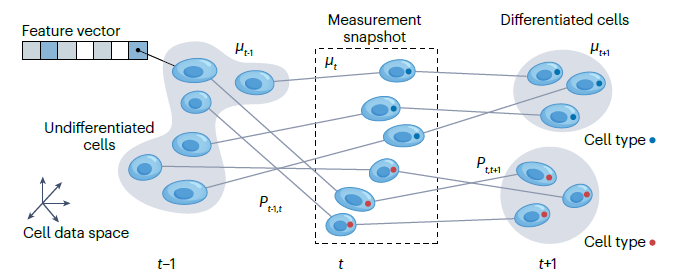
\includegraphics[width=0.65\textwidth]{cell_differentiation.png}
			\caption{Cell differentiation relationship. \cite{bunne2024optimal}}
		\end{figure}
	\end{frame}
	
	
		
		\begin{frame}
			\frametitle{Optimal Transport: A Flexible Alternative}
\begin{itemize}
	\item \textbf{Why Use OT for Single-Cell Comparison?}
	\begin{itemize}
		\item Flexible cost functions to transition between cell expression profiles.
		\item Models biologically relevant transitions in gene pathways and cellular dynamics.
	\end{itemize}
	
	\item \textbf{Context}:
		\begin{itemize}
			\item Interested in the evolution of cell populations.
			\item OT allows adjustments to the cost matrix, aligning transformation likelihood with gene expression changes.
		\end{itemize}
	\end{itemize}
		\end{frame}
		
		\begin{frame}
			\frametitle{Motivating Example: Gene Interaction in Immune Response}
			\begin{itemize}
				\item \textbf{Gene A (Cytokine Receptor)}:
				\begin{itemize}
					\item Essential for receiving environmental signals—low cost in transitions.
				\end{itemize}
				
				\item \textbf{Gene B (Transcription Factor)}:
				\begin{itemize}
					\item Works closely with Gene A to activate immune response genes—low joint transformation cost with Gene A.
				\end{itemize}
				
				\item \textbf{Gene C (Cell Surface Marker)}:
				\begin{itemize}
					\item Expression increases in activated cells but costly to adjust in conjunction with B or A independently.
					\item Higher transformation cost with both A and B reflects its distinct biological role.
				\end{itemize}
				
				\item \textbf{Biological Insight}:
					\begin{itemize}
						\item Shows how OT can prioritize coupled transformations within a pathway (A \& B) while maintaining overall functional coherence by recognizing C's selective role.
					\end{itemize}
				\end{itemize}
			\end{frame}
			
			\begin{frame}
				\frametitle{Interpreting OT in Single-Cell Context}
				\begin{itemize}
					\item \textbf{OT Advantages}:
						\begin{itemize}
							\item Enables comparisons considering gene-specific contexts and evolutionary pathways.
							\item Cost matrix adjustments reflect biological transformation costs, aligning with cellular evolution likelihood.
						\end{itemize}
					\end{itemize}
					\begin{figure}
						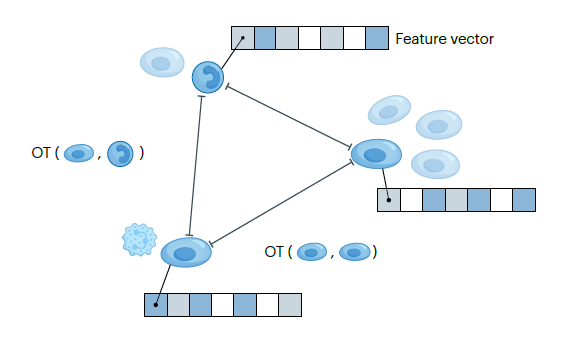
\includegraphics[width=0.5\textwidth]{single_cell.png}
						\caption{OT distances for cells. \cite{bunne2024optimal}}
					\end{figure}
				\end{frame}
	
	% Applications to Spatial Omics
	\subsection{Applications to Spatial Omics}
	\begin{frame}
		\frametitle{Spatial Omics: Research Questions}
		\begin{itemize}
				
				\item \textbf{Key Biological Questions}:
				\begin{itemize}
					\item Understanding cell–cell communication and spatial distribution of molecules.
					\item Identifying key structural and functional units like microenvironments (MEs) and niches.
				\end{itemize}
			\end{itemize}
		\end{frame}
		
		\begin{frame}
			\frametitle{Optimal Transport in Spatial Omics}
			\begin{itemize}
				\item \textbf{Using OT for Analyzing Microenvironments}:
					\begin{itemize}
						\item OT distance for analysis of multicellular communities.
						\item Models the microenvironment (ME) around each cell by aggregating spatial neighbor features into histograms.
					\end{itemize}
					
					\item \textbf{Computational Approach}:
					\begin{itemize}
						\item Compute OT distance between MEs: \(OT(ME_i, ME_j)\).
						\item Forms a pairwise distance matrix for all cellular MEs.
					\end{itemize}
				\end{itemize}
				\begin{figure}
					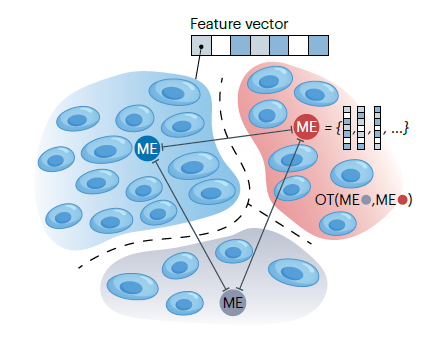
\includegraphics[width=0.45\textwidth]{spatial1.png}
					\caption{OT distances of MEs. \cite{bunne2024optimal}}
				\end{figure}
			\end{frame}
			
			\begin{frame}
				\frametitle{Applications and Biological Insights}
				\begin{itemize}
					\item \textbf{Clustering of Microenvironments}:
						\begin{itemize}
							\item Apply clustering on the OT-derived distance matrix to identify cellular niches.
						\end{itemize}
						
						\item \textbf{Real-World Findings}:
							\begin{itemize}
								\item Studies by Yuan et al. and Mani et al. exemplify the use of OT in spatial omics.
								\item OT-based MEs resemble known tissue structures when using multiplex fluorescence data.
							\end{itemize}
							
							\item \textbf{Visual Confirmation}:
								\begin{itemize}
									\item Detected microenvironments align with ground-truth tissue sections, corroborating OT's efficacy in characterizing spatial structures.
								\end{itemize}
							\end{itemize}
							\begin{figure}
								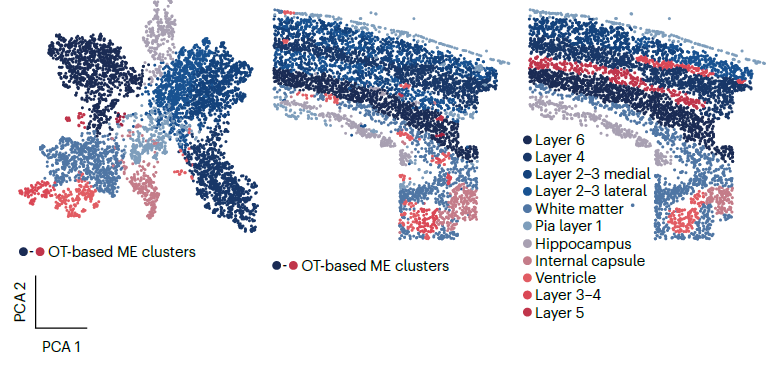
\includegraphics[width=0.4\textwidth]{spatial2.png}
								\caption{Clustering visualization of MEs. \cite{bunne2024optimal}}
							\end{figure}
						\end{frame}
						
	
	% scDiagnostics in Bioconductor
	\section{Optimal Transport in \texttt{scDiagnostics}}
	
	\begin{frame}
		\frametitle{Optimal Transport in \texttt{scDiagnostics}}
		\begin{itemize}
			\item \textbf{Purpose}:
			\begin{itemize}
				\item Calculates Wasserstein distances (another name for Kantorovich distances) between query and reference single-cell datasets.
			\end{itemize}
			
			\item \textbf{Process Overview}:
			\begin{itemize}
				\item Projects query data into PCA space defined by the reference dataset.
				\item Computes Wasserstein distances within the reference dataset to establish a null distribution.
				\item Assesses differences by calculating distances between the query and reference datasets.
			\end{itemize}
			\item \textbf{Biological Context}:
			\begin{itemize}
				\item Identifies variations in cell populations or expression profiles.
			\end{itemize}
		\end{itemize}
	\end{frame}
	
	\begin{frame}
		\frametitle{Optimal Transport in \texttt{scDiagnostics}}
		\begin{itemize}
			\item \textbf{Biological Context}:
				\begin{itemize}
					\item Identifies variations in cell populations or expression profiles.
					\item Provides insights into cell type differentiation and evolutionary pathways.
				\end{itemize}
				
				\item \textbf{Key Outputs}:
					\begin{itemize}
						\item \texttt{null\_dist}: A numeric vector of distances from resampled reference dataset pairs.
						\item \texttt{query\_dist}: Mean distance between the query and reference datasets.
						\item \texttt{cell\_type}: Lists unique cell types identified in the reference dataset.
					\end{itemize}
				\end{itemize}
			\end{frame}
			
			\begin{frame}
				\frametitle{Optimal Transport in \texttt{scDiagnostics} Example}
				\begin{itemize}
					\item \textbf{Data Preparation}:
					\begin{itemize}
						\item Load \texttt{reference\_data} and \texttt{query\_data}.
						\item Select CD4 cells from both datasets.
					\end{itemize}
					
					\item \textbf{Gene Selection}:
					\begin{itemize}
						\item Extract top 500 highly variable genes and find common genes.
					\end{itemize}
					
					\item \textbf{Dimensionality Reduction}:
					\begin{itemize}
						\item Perform PCA on reference data for feature reduction.
					\end{itemize}
					
					\item \textbf{OT Distance Calculation}:
					\begin{itemize}
						\item Compute Wasserstein distances and evaluate differences.
					\end{itemize}
					
					\item \textbf{Visualization}:
					\begin{itemize}
						\item Plot to compare datasets.
					\end{itemize}
					
					\item \textbf{Output}:
					\begin{itemize}
						\item See code example in \texttt{R} script.
					\end{itemize}
				\end{itemize}
			\end{frame}
			
	
	% Conclusion
	\section{Conclusion}
	\begin{frame}
		\frametitle{Conclusion}
		\begin{itemize}
			\item \textbf{Optimal Transport (OT)}:
			\begin{itemize}
				\item Provides a versatile framework for comparing complex biological data.
			\end{itemize}
			
			\item \textbf{Single-Cell Analysis}:
				\begin{itemize}
					\item Offers a flexible approach to understand cell-type differences and evolutionary dynamics.
				\end{itemize}
				
				\item \textbf{Spatial Omics}:
					\begin{itemize}
						\item Enables characterization of microenvironments, revealing key tissue structures.
					\end{itemize}
					
					\item \textbf{Broader Impact}:
						\begin{itemize}
							\item OT bridges gaps between computational methods and biological insights, driving advances in multi-omics research.
						\end{itemize}
					\end{itemize}
				\end{frame}
				
	% References
	\section{References}
	\begin{frame}[allowframebreaks]
		\frametitle{References}
		\printbibliography
	\end{frame}
	
\end{document}